\documentclass{article}
\usepackage[utf8]{inputenc}
\usepackage{graphicx} % Required for inserting images
\usepackage{pgfplots}

\title{graficas}
\author{Matías Cejas}
\date{December 2023}

\pgfplotsset{compat=1.18, width=14.5cm}
\begin{document}


\section{Gráfica solución EDO}
%FUNCION REAL
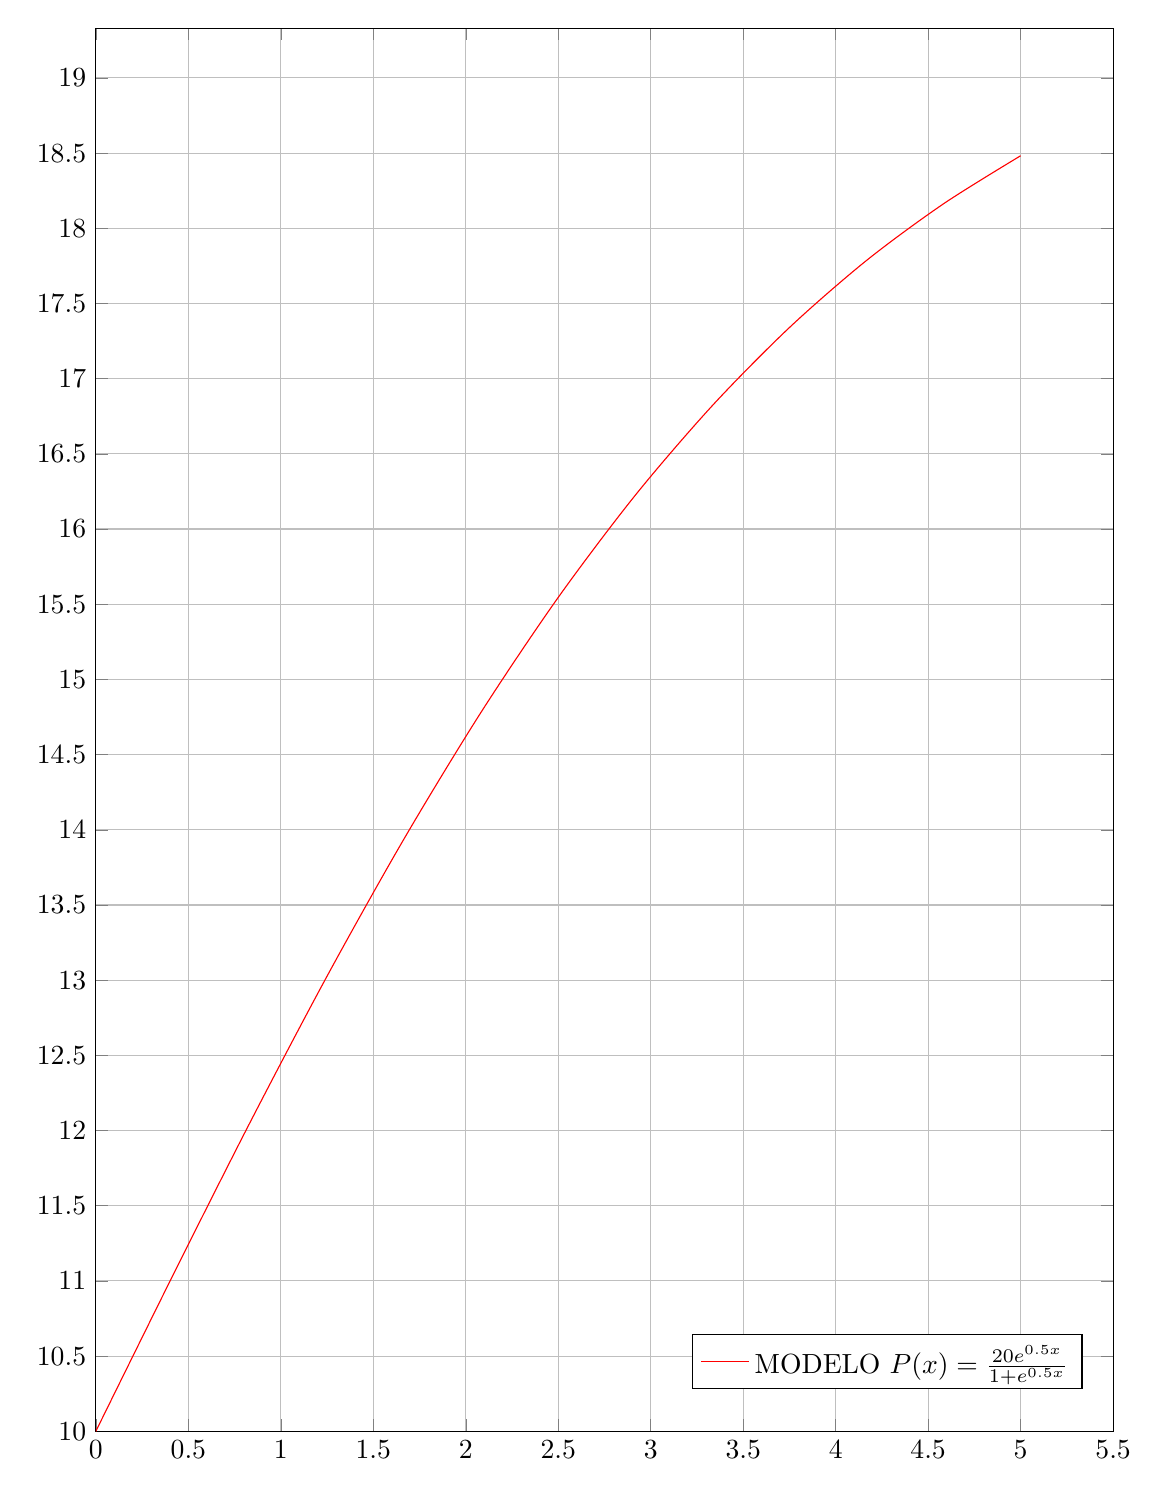
\begin{tikzpicture}
\begin{axis}[legend pos=south east,grid=major, height=1.6\textwidth,xmin=0,ymin=10]
\addplot[smooth,color=red]{ 20*e^(0.5*x)/(1+e^(0.5*x))};
\addlegendentry{MODELO $P(x)=\frac{20e^{0.5x}}{1+e^{0.5x}}$}
\end{axis}
\end{tikzpicture}

%ZOOM SECCION APROXIMADA
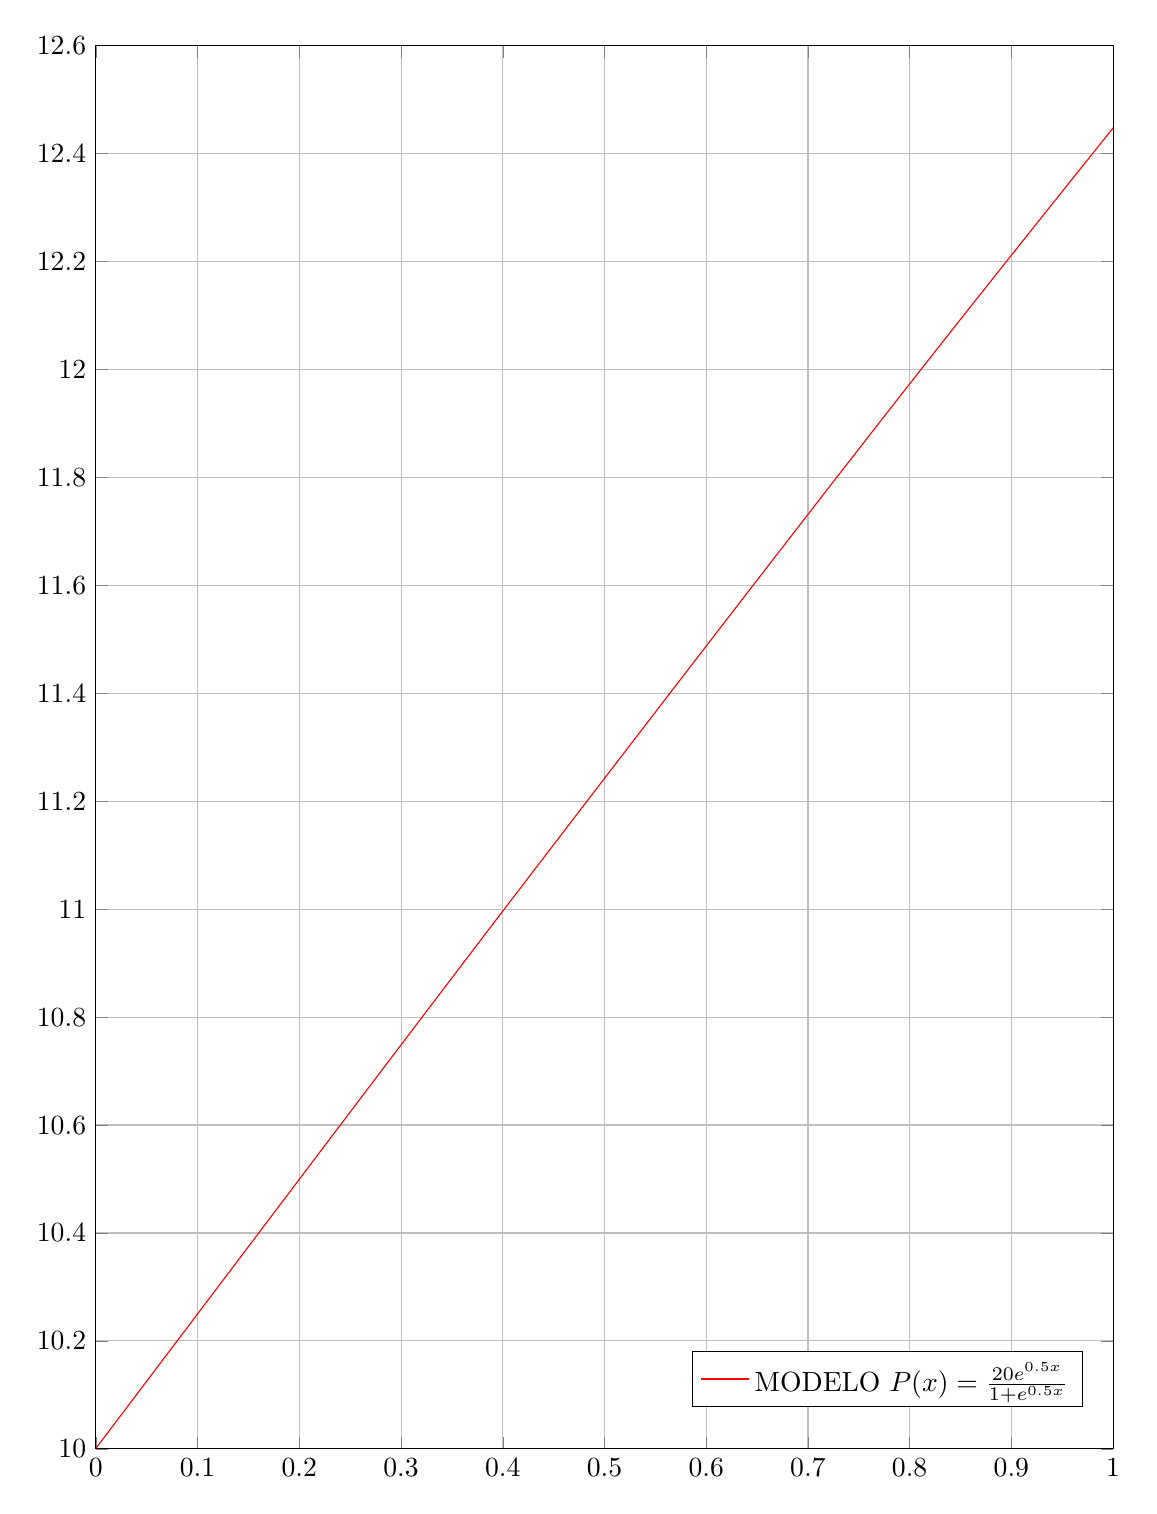
\begin{tikzpicture}
\begin{axis}[legend pos=south east,grid=major, height=1.6\textwidth,xmin=0,ymin=10,ymax=12.6,xmax=1]
\addplot[smooth,color=red]{ 20*e^(0.5*x)/(1+e^(0.5*x))};
\addlegendentry{MODELO $P(x)=\frac{20e^{0.5x}}{1+e^{0.5x}}$}
\end{axis}
\end{tikzpicture}

\section{Gráfica Euler}
%EULER 0.1
\begin{tikzpicture}
\begin{axis}[legend pos=south east, grid=major, height=1.6\textwidth,xmin=0,xmax=1,ymin=10,ymax=12.5]
\addplot+[draw=red,mark=asterisk,mark size=2pt]
table[meta=pi]
{EULER1A.txt};
\addlegendentry{ESTIMACIÓN EULER H=0.1}[]
\end{axis}
\end{tikzpicture}

%EULER 0.05
\begin{tikzpicture}
\begin{axis}[legend pos=south east, grid=major, height=1.6\textwidth,xmin=0,xmax=1,ymin=10,ymax=12.6]
\addplot+[draw=blue,mark=asterisk,mark size=2pt]
table[meta=pi]
{EULER1B.txt};
\addlegendentry{ESTIMACIÓN EULER H=0.05}
\end{axis}
\end{tikzpicture}

%EULER 0.02
\begin{tikzpicture}
\begin{axis}[legend pos=south east, grid=major, height=1.6\textwidth,xmin=0,xmax=1,ymin=10,ymax=12.6]
\addplot+[draw=orange,mark=|,mark size=2pt]
table[meta=pi]
{EULER1C.txt};
\addlegendentry{ESTIMACIÓN EULER H=0.02}]
\end{axis}
\end{tikzpicture}


\section{Gráfica comparación Euler}
%Comparacion
\begin{tikzpicture}
\begin{axis}[legend pos=south east, grid=major, height=1.6\textwidth,xmin=0,xmax=1,ymin=10,ymax=12.6]
\addplot+[draw=red,mark=asterisk,mark size=2pt]
table[meta=pi]
{EULER1A.txt};
\addlegendentry{ESTIMACIÓN EULER H=0.1}[]
\addplot+[draw=blue,mark=asterisk,mark size=2pt]
table[meta=pi]
{EULER1B.txt};
\addlegendentry{ESTIMACIÓN EULER H=0.05}
\addplot+[draw=orange,mark=|,mark size=2pt]
table[meta=pi]
{EULER1C.txt};
\addlegendentry{ESTIMACIÓN EULER H=0.02}
\end{axis}
\end{tikzpicture}

\section{Heun}
%HEUN 0.1 SOLO
\begin{tikzpicture}
\begin{axis}[legend pos=south east, grid=major, height=1.6\textwidth,xmin=0,xmax=1,ymin=10,ymax=12.6]
\addplot+[draw=red,mark=asterisk,mark size=2pt]
table[meta=pi]
{HEUN1A.txt};
\addlegendentry{ESTIMACIÓN HEUN H=0.1}[]
\end{axis}
\end{tikzpicture}
%HEUN 0.05 SOLO
\begin{tikzpicture}
\begin{axis}[legend pos=south east, grid=major, height=1.6\textwidth,xmin=0,xmax=1,ymin=10,ymax=12.6]
\addplot+[draw=blue,mark=asterisk,mark size=2pt]
table[meta=pi]
{HEUN1B.txt};
\addlegendentry{ESTIMACIÓN HEUN H=0.05}[]
\end{axis}
\end{tikzpicture}
%HEUN 0.02 SOLO
\begin{tikzpicture}
\begin{axis}[legend pos=south east, grid=major, height=1.6\textwidth,xmin=0,xmax=1,ymin=10,ymax=12.6]
\addplot+[draw=orange,mark=asterisk,mark size=2pt]
table[meta=pi]
{HEUN1C.txt};
\addlegendentry{ESTIMACIÓN HEUN H=0.02}[]
\end{axis}
\end{tikzpicture}

\section*{Comparación HEUN TODAS}
\begin{tikzpicture}
\begin{axis}[legend pos=south east, grid=major, height=1.6\textwidth,xmin=0,xmax=1,ymin=10,ymax=12.6]
\addplot+[draw=red,mark=asterisk,mark size=2pt]
table[meta=pi]
{HEUN1A.txt};
\addlegendentry{ESTIMACIÓN HEUN H=0.1}[]

\addplot+[draw=blue,mark=asterisk,mark size=2pt]
table[meta=pi]
{HEUN1B.txt};
\addlegendentry{ESTIMACIÓN HEUN H=0.05}[]

\addplot+[draw=orange,mark=asterisk,mark size=2pt]
table[meta=pi]
{HEUN1C.txt};
\addlegendentry{ESTIMACIÓN HEUN H=0.02}[]

\end{axis}
\end{tikzpicture}










\section*{Comparación Euler y Heun}
%EULER Y HEUN
\begin{tikzpicture}
\begin{axis}[legend pos=south east, grid=major, height=1.6\textwidth,xmin=0,xmax=1,ymin=10,ymax=12.6]
\addplot+[draw=orange,mark=asterisk,mark size=2pt]
table[meta=pi]
{EULER1C.txt};
\addlegendentry{ESTIMACIÓN EULER H=0.02}[]
\addplot+[draw=violet,mark=asterisk,mark size=2pt]
table[meta=pi]
{HEUN1C.txt};
\addlegendentry{ESTIMACIÓN HEUN H=0.02}[]

\end{axis}
\end{tikzpicture}

\end{document}